\chapter{Introduction}
\label{chap:introduction}


Maps are the main tool to represent geographical information.
As geographical information is usually scale-dependent
\parencite{Weibel1997},
users need to have access to maps of different scales.
Producing these maps independently is
time-consuming and labor-intensive.
A better strategy is 
to collect data at a large scale by surveying, 
and then to derive maps 
at smaller scales from the large-scale map.
This kind of deriving is known as \emph{map generalization}
\parencite{Li2007}.
More specifically, map generalization is 
the process of extracting and rearranging 
the geographical information of a larger-scale map 
in order to produce smaller-scale maps.
A requirement of map generalization is to emphasize the 
essential while suppress the unimportant,
and at the same time maintain logical relationship between 
objects \parencite{Weibel1997}.
As manual generalization is still a lot of work for human being
\parencite{Duchene2014},
automating map generalization is a promising way 
to produce up-to-date maps at high speed and low cost 
\parencite{Mackaness2017Generalization}.


In our digital age, people interactively read maps 
on computers and mobile phones.
An often used interaction is zooming. 
When users zoom in or out, 
a map must be changed to provide information 
appropriate to the corresponding zoom level.
A naive solution is 
to switch between maps at different scales.
A more advanced strategy to support zooming is  
on-the-fly generalization,
which emphasizes on generalizing in real time
\parencite{Weibel2017Fly}.
These methods, however, can result in discrete changes, which
tend to distract users.
To have a better zooming experience, 
users expect the changes to be continuous.
This is why some digital maps such as Google Maps 
are trying to make zooming as continuous as possible.
The process of producing maps at different scales
with smooth changes 
is called \emph{continuous map generalization},
or briefly continuous generalization
\parencite{Sester2005_CG}.
Ideally, there should be no discrete change 
in continuous generalization.
However, the term is used when 
the discrete changes are small enough,
e.g., \textcite{Suba2016Road}.



\section{State of the Art}
\label{sec:Intro_State}


Map generalization takes into account requirements
in order to produce maps with high quality.
We categorize these requirements as hard constraints 
and soft constraints.
For example, when users zoom out, 
some land cover areas become too small to be seen.
These areas have to be aggregated.
When we aggregate an area into another area, the type of the 
former area is changed to the type of the later one. 
In this problem a hard constraint can be that we aggregate only 
two polygons at each step in order to keep changes small
(see for example \fig\ref{fig:Intro_SubdivisionName}). 
A soft constraint can be that we wish to minimize the changes of 
types, e.g., we prefer aggregating a grass area into a farm 
area rather than into a settlement area.
This is a typical \emph{optimization} problem,
where we stick to hard constraints and 
try to fulfill soft ones as good as possible.
Optimization for map generalization is important 
not only because it finds optimal solutions,
but also because it evaluates the quality of a model
\parencite{Haunert2011Benchmark}.
Recall that we wish to minimize the changes of types
when aggregating areas one by one.
A model can be to minimize 
the smallest change over all the steps.
Instead, an other model can be to minimize 
the average change over all the steps.
Using optimization, we are able to find best solutions 
from both the models.
Then we can evaluate the models based on their best solutions.
Moreover, optimization is useful for evaluating heuristics.
We need heuristics because
many optimization problems cannot be solved efficiently
\parencite[e.g.,][]
{HaunertWolff2010AreaAgg,Chimani2014Eat,Haunert2016Partition}.
While heuristics can find some solutions in reasonable time,
it is important to know the quality of 
these solutions.
Fortunately, we can often find an optimal solution when 
the size of an instance is sufficiently small.
Consequently, we can evaluate the quality of a heuristic by
comparing its results with optimal solutions
on small instances.

\begin{figure}[tb]
	\centering
	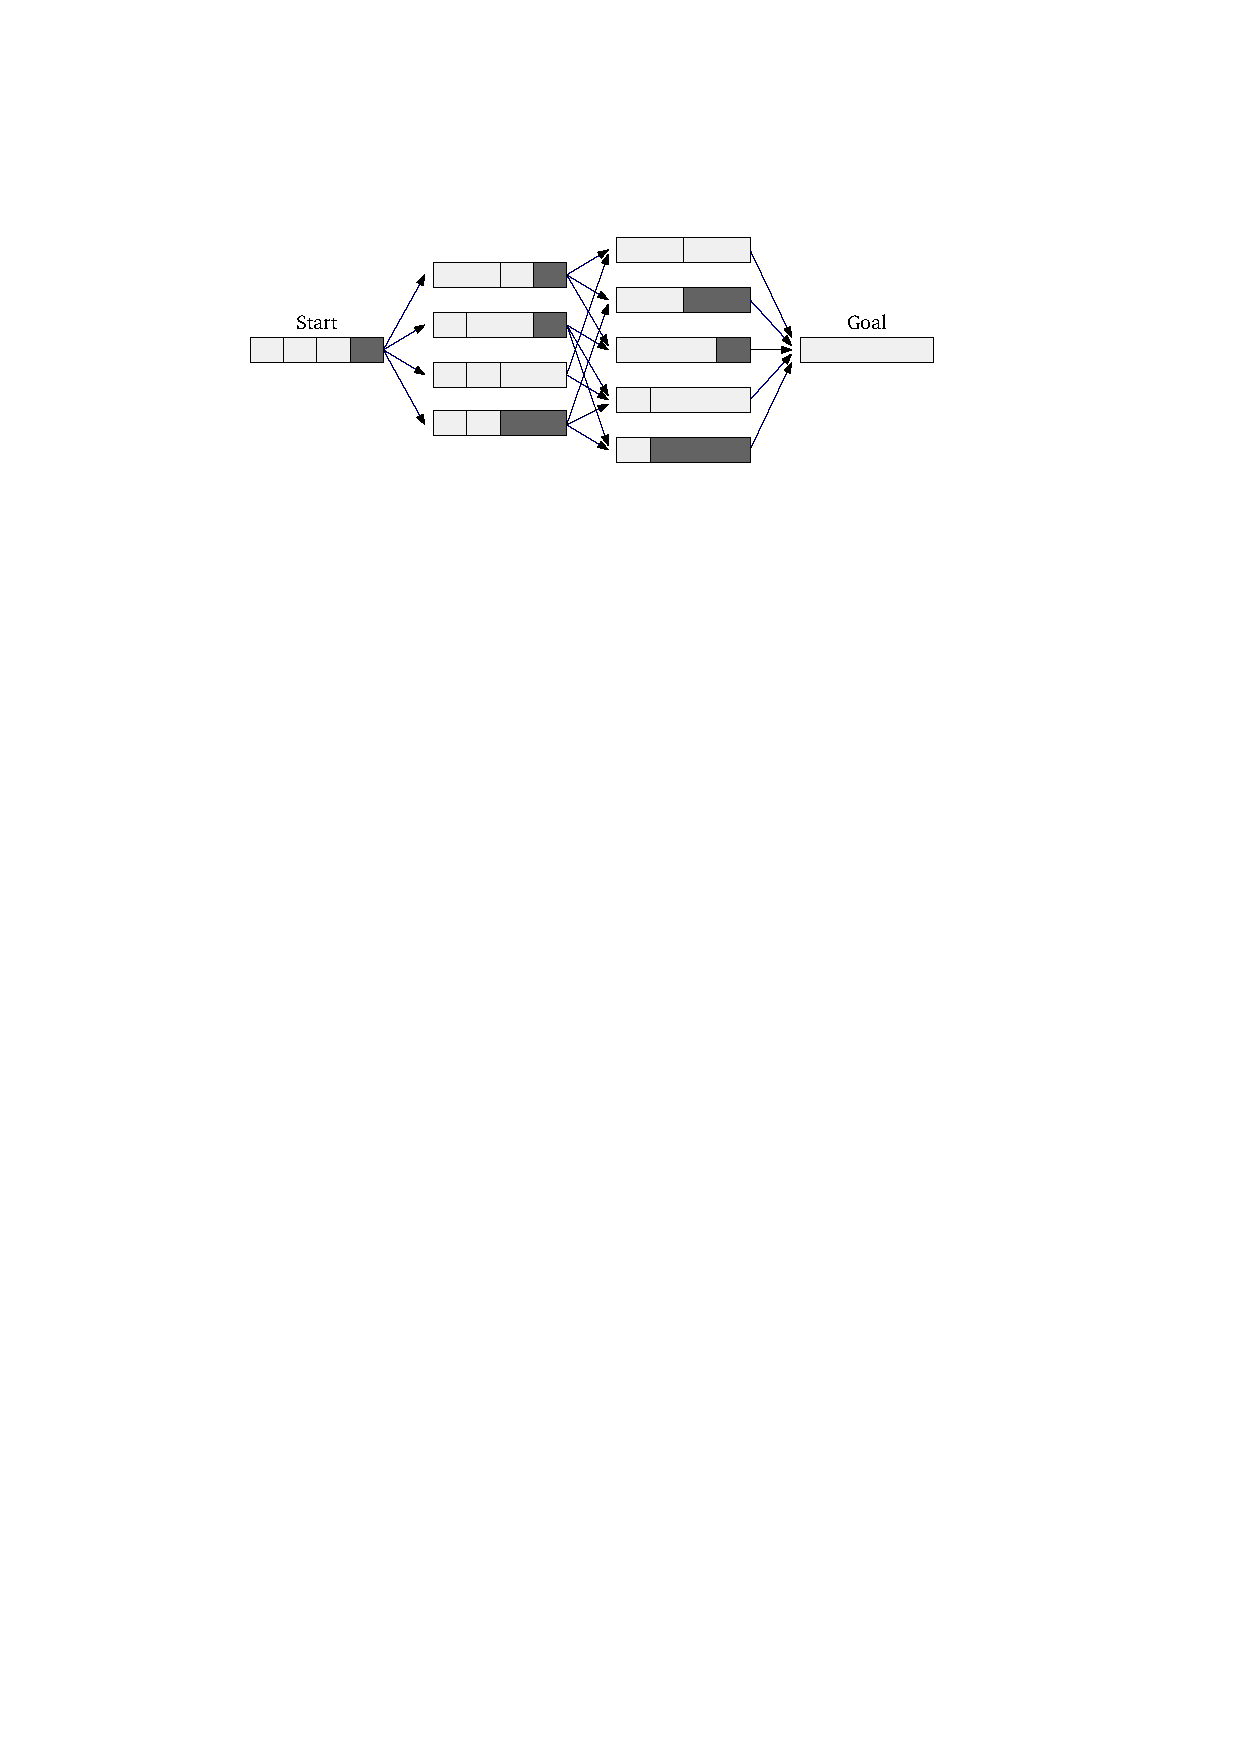
\includegraphics[page=1]{Intro}
	\caption{There are many ways of aggregating a set of land 
	cover areas to a single one.}
	\label{fig:Intro_SubdivisionName}
\end{figure}

Optimization has been widely used in map generalization.
For example, \textcite{Harrie1999} displaced objects based on 
least-squares adjustment (LSA) to solve spatial conflicts
(for a brief recap of LSA, see \sect\ref{sec:Intro_Tools}).
In their problem, the soft constraints 
of shapes and locations may contradict each other.
The best solution is to find a compromise that satisfies the 
constraints as much as possible. 
Such a compromise can be found by LSA.
\textcite{Sester2005Optimization} used LSA not only for 
displacing objects, but also for simplifying buildings, 
where the boundaries of the simplified versions were required to 
be as close as possible to the original buildings.
\textcite{Regnauld2001} grouped buildings based on 
a minimum spanning tree in order to do a typification of 
the buildings in the same group.
\textcite{HaunertWolff2010AreaAgg} aggregated land cover areas
based on mixed-integer linear programming,
which we briefly introduce in \sect\ref{sec:Intro_Tools}.
They wanted to minimize the changes of types and maximize the 
compactnesses of shapes.
\textcite{Haunertwolff2010Building} simplified building
footprints by solving an integer linear program.
They aimed at minimizing the number of edges in the output under 
the restriction that the simplified buildings must be 
topologically safe,
that is, the selected and extended edges must not intersect with 
each other.



Optimization becomes more delicate
when we deal with \emph{continuous} map generalization.
In this area, we have requirements 
not only for a specific map, 
but also for relations between maps. 
For example, in \fig\ref{fig:Intro_SubdivisionName} two 
aggregated polygons should not be separated at later steps. 
%
Some optimization techniques have been applied in 
continuous map generalization. 
\textcite{Noellenburg2008} used 
dynamic programming (see \sect\ref{sec:Intro_Tools})
to match points of two polylines to support morphing.
Their objective was to minimize some cost of the matching.
\textcite{sahw-oarps-ICAGW13} used mixted-integer linear 
programming to select points of interest.
They required that 
a disappeared point should not show up again during zooming out, 
and any two points should be 
sufficiently far away from each other.
Based on these requirements, they wanted to show as many points 
as possible when zooming out.
\textcite{Chimani2014Eat} computed a deletion sequence
for a road network by integer linear programming.
They wanted to delete a stroke, 
which is a sequence of edges, at each step,
while keeping the remaining network connected.
They assigned each edge a weight, 
and their objective was to maximize the overall weights of all 
the road networks.

\section{Tools for Optimization}
\label{sec:Intro_Tools}

In this thesis, we use some well-known optimization methods,
namely,
the \Astar algorithm \parencite{Hart1968}, 
integer linear programming
\parencite[chapter~13]{Papadimitriou1982combinatorial},
dynamic programing \parencite[chapter~15]{Cormen2009}, and
least-squares adjustment (LSA) \parencite[chapter~3]{Koch1988}.
We also use the minimum spanning tree;
see \parencite[chapter~23]{Cormen2009}.
%
We use \Astar and integer linear programming in order 
to compute optimal sequences for 
area aggregation (see \chap\ref{chap:AreaAgg}).
Similar to \textcite{Noellenburg2008},
we use dynamic programming to 
compute corresponding points between polylines
(see \chaps\ref{chap:Admin} and \ref{chap:Morph}).
We use the minimum spanning tree to group buildings,
which is similar to \textcite{Regnauld2001}; see \chap\ref{chap:Bldg}.
We define trajectories based on LSA 
for morphing between polylines (see \chap\ref{chap:Morph}).
% There is no optimization used in \chap\ref{chap:DataStr}.
In the following, we briefly recall these methods.


Given a graph with nodes and weighted edges,
a typical task is to find a shortest path 
from a start node to a goal node.
A breadth-first search \parencite[chapter~22]{Cormen2009}
solves the shortest-path problem 
in unweighted graphs.
Dijkstra's algorithm \parencite{Dijkstra1959}
always chooses 
from the explored nodes the neighbor 
with minimum distance from the start node. 
The \Astar algorithm is 
a generalized version of Dijkstra's algorithm.
When \Astar chooses a node to explore the neighbors,
the algorithm not only takes into account 
the distance from the start node,
but also estimates the distance to the goal node.
By always choosing a node which is likely 
to be closer to the goal node, 
\Astar often explores fewer nodes than Dijkstra's algorithm
in finding a shortest path.
If the estimated distance is always smaller than the exact 
distance to the goal node, 
the path found by \Astar is guaranteed to be shortest.

Linear programming models an optimization problem as objective 
functions subject to constraints,
where the objective functions and constraints are represented by 
linear functions of some variables.
These constraints form a convex polyhedron.
An optimal solution lies on the boundary of the polyhedron and 
can be found efficiently.
\emph{Integer} linear programming requires that
the variables must use integers.
Integer linear programming is NP-hard
since many NP-hard problems such as vertex cover can be 
formulated as integer linear programs.
Intuitively, this is due to the fact that the optimal solution 
may lie in the interior of the polyhedron, where geometry does 
not help to find it.
If only some of the variables are required to be integers
and other variables are allowed to be non-integers, 
then the problem is called mixed integer linear programming,
which is also known as NP-hard; see for more details
\textcite[chapter~16]{Schrijver1986}.



Dynamic programming decomposes 
a big instance of a complex problem 
into a collection of smaller subinstances.
The method solves each subinstance just once and saves the 
solution. 
The next time when the same subinstance occurs, the solution of 
the subinstances will be used instead of resolving this 
subinstance. 
In this way, computation time can be saved.
Other than in the divide-and-conquer approach used, 
e.g., in merge sort, 
in dynamic programming subinstances of equal size 
are usually \emph{not} disjoint, but overlap.

Least squares adjustment is a model for solving 
over-constrained problems.  
There are a set of unknowns and a set of observations.
The objective is to calculate the unknowns based on the 
observations.
Because of errors, the observations may contradict each other.
We have to make some adjustments for the 
observations so that there is a set of unknowns that agree 
all the adjusted observations.
There can be infinitively many sets of adjustments feasible, 
but we choose the one with the least sum of squares.
Based on this set of adjustments,
we can finally compute the unknowns.



Given a graph with nodes and weighted edges, 
a minimum spanning tree (MST) of the graph is a minimum-weight subset
of the edges that together connect all nodes.
Surprisingly, the MST can be computed by simple greedy algorithms
such as Kruskal's algorithm \parencite{Kruskal1956}
or the algorithm of Jarn\'ik--Prim \parencite{Jarnik1930,Prim1957}.
Strictly speaking, the MST by itself is not an optimization
\emph{method}, but it is a helpful structure of low weight that helps
to solve many optimization problems in graph theory at least
approximately, for example, the metric version of the famous Traveling
Salesperson Problem (TSP).


\section{Overview of the Thesis}
\label{sec:Intro_Overview}

This thesis contains five chapters that deal with methods for 
continuous 
generalization. 
First, we consider the problem of finding 
optimal sequences for aggregating land-cover areas.
%
Second, we continuously generalize county boundaries to
provincial boundaries.
%
Third, we generalize buildings to built-up areas 
by aggregating and growing.
%
Fourth, we define moving trajectories
based on least-squares adjustment
for morphing between polylines.
%
Fifth, we discuss the performance 
of data structures for spatial problems.
In the remainder of this section, 
we present our results in more detail.


\subsubsection{Finding Optimal Sequences for Area Aggregation -- 
\protect \\ \Astar vs. Integer Linear Programming}

Given two land-cover maps of different scales, 
we wish to find a sequence of small incremental
changes that gradually transforms one map into the other.
We assume that the two input maps consist of
polygons that constitute a planar subdivision and belong to
different land-cover classes. 
Every polygon in the smaller-scale map
is the union of a set of polygons in the larger-scale map. 
In each step of the sequence that we compute, 
the smallest area is merged with one of its neighbors. 
We do not select that neighbor according to a prescribed rule 
but define the whole sequence of pairwise merges at once, 
based on global optimization.
We formalize this problem as 
finding a shortest path in a graph.
We compare finding optimal solutions by the \Astar algorithm 
and integer linear programming.
In addition, we present a greedy algorithm 
as a benchmark.
We tested the three methods with a
dataset of the official German topographic database ATKIS.
The main result is that 
\Astar finds better solutions than the other two methods.
\fig\ref{fig:Intro_AreaAgg_Case612} shows some intermediate 
results obtained by \Astar for one of the regions.
This is joint work with Alexander Wolff and Jan-Hendrik Haunert,
part of which has been published \cite{Peng2017AStar}.


\begin{figure}[tb]
	\centering
	\includegraphics[page=2]{Intro}
	\caption{Some intermediate aggregation results of 
		a region (Buchholz in der Nordheide, Germany). 
		There are $9$ polygons on 
		the larger-scale map (top left). 
		These areas are aggregated into one 
		on the smaller-scale map (bottom left). 
		The digits are the numbers of the areas.
}
	\label{fig:Intro_AreaAgg_Case612}
\end{figure}

\subsubsection{Generalizing Administrative Boundaries
	Based on Compatible Triangulations}

Topological consistency is a key issue 
in cartographic generalization.
Our aim in this chapter is to ensure topological consistency  
during continuous generalization of administrative boundaries.
Tho this end, we present a five-step method.
We assume that we have two maps of administrative
boundaries at different scales, where the larger-scale map has 
not
only more details but also an additional level of administrative
regions.

Our main contribution is the proposal of a workflow for
generalizing hierarchical administrative boundaries in a
continuous and topologically consistent way.  First, we
identify corresponding boundaries between the two maps.
We call the remaining boundary pieces (on the larger-scale map)
\emph{unmatched} boundaries.  Second, we use a method based on 
compatible triangulations to generate
additional boundaries for the smaller-scale map that correspond 
to the
unmatched boundaries.  
Third, we simplify the resulting additional boundaries
by Douglas--Peukcer algorithm.  
Fourth, we compute corresponding points for each pair
of corresponding boundaries using a variant of an existing 
dynamic programming algorithm.  
Fifth, we interpolate between the corresponding points
to generate the boundaries at intermediate scales.

We do a thorough
case study based on the provinces and counties of Mainland China.
Although topologically consistent algorithms for the third step 
and the
fifth step exist, we have implemented simpler algorithms for our
case study. 
\fig\ref{fig:Intro_AdminBound_Tianjin} shows our results of 
continuously generalizing county boundaries 
to provincial boundaries of Tianjin, China.
This is joint work with Alexander Wolff and Jan-Hendrik Haunert
\cite{Peng2016Admin}.

\begin{figure}[tb]
	\centering
	\includegraphics[page=3]{Intro}
	\caption{Continuously generalizing county boundaries to 
	provincial boundaries of Tianjin province, China.}
	\label{fig:Intro_AdminBound_Tianjin}
\end{figure}

\subsubsection{Generalizing Buildings to Built-up Areas 
	by Aggregating and Growing}

To enable smooth zooming, we propose a method to continuously 
generalize buildings from a given start map to a smaller-scale 
goal map, where 
there are only built-up area polygons instead of individual 
building polygons
(see Figure~\ref{fig:Intro_BldgGrow}).
We name the buildings on the start map \emph{original buildings}.
%
For an intermediate scale, 
we aggregate the original buildings that will become too close 
by adding bridges.
We grow (bridged) original buildings based on buffering, 
and simplify the grown buildings.
We take into account the shapes of the buildings 
both at the previous map and goal map to make sure that 
the buildings are always growing.
The running time of our method is in $O(n^3)$,
where $n$ is the total number of edges
overall the original buildings.
%

The advantages of our method are as follows. 
First, the buildings grow continuously 
and, at the same time, are simplified.
Second, right angles of buildings are preserved during growing: 
the merged buildings still look like buildings. 
Third, the distances between buildings are 
always larger than a specified threshold.
We do a case study to show the performances of our method.
This is joint work with Guillaume Touya~\cite{Peng2017Building}.

\begin{figure}[tb]
	\centering
%	\includegraphics[page=4]{Intro}
	\includegraphics[page=4]{Bldg_CaseStudy_DataAndResults}
	\caption{Continuously generalizing buildings to built-up 
		areas by aggregating and growing.}
	\label{fig:Intro_BldgGrow}
\end{figure}

\subsubsection{Morphing Polylines Based on Least-Squares 
Adjustment}

One way to achieve continuous generalization of polylines is to 
use morphing 
techniques. 
Most often for morphing, the vertices of the polylines move on 
defined 
straight-line trajectories at constant speeds.
In this chapter we address morphing of polylines, but we relax 
the requirement 
that the vertices of the polylines move on straight lines. Our 
concern with 
straight-line trajectories is that characteristic properties of 
the polylines 
change drastically during the morphing process. In particular, 
we suggest that 
the angles and edge lengths of the polylines should change 
linearly during the 
morphing process. This expectation is clearly not accomplished 
with 
straight-line trajectories. In contrast, we present a new method 
based on 
least-squares adjustment that yields close-to-linear changes of 
the angles and 
edge lengths. 
Figure~\ref{fig:Intro_LSA_Compare} shows a comparison of 
morphing based on 
straight-line trajectories and our new morphing method.
This is joint work with Jan-Henrik Haunert,
Alexander Wolff, and Christophe Hurter~\cite{Peng2013LSA}.

\begin{figure}[htb]
	\centering
	\includegraphics[page=2]{Morph_CaseStudy_Artificial}
	\caption{A comparison of morphing based on the two different 
	trajectories.}
	\label{fig:Intro_LSA_Compare}
\end{figure}

\subsubsection{Choosing the Right Data Structures for Solving 
Spatial Problems}

When we plan to implement a program, 
there are always many data structures that
we can use to achieve a certain goal.
However, the program may be inefficient
if the data structures are not chosen and used carefully.
As an example, we consider the problem of 
finding pairs of close points from a dataset. 
We consider two points to be close 
if they lie within a square of pre-specified 
side length $\varepsilon$. 
We compare three obvious algorithms to solve the problem: 
a sweep-line (SL) algorithm, 
an algorithm based on the Delaunay triangulation (DT) 
of the input points, 
and a hashing-like algorithm 
which overlays the input points with a rectangular grid. 
We implemented the algorithms in C\# and tested them on 
randomly generated data and real-world data. 
We used the DT available in ArcGIS Objects. 
We used three different \emph{balanced binary search} 
tree data structures, 
i.e., SortedDictionary (SD), SortedSet (SS), and TreeSet (TS), 
to implement the sweep-line algorithm. 
However, the simple grid-based algorithm 
turned out to run faster than 
any of the other algorithms 
by a factor of at least $2$ 
(see Figure~\ref{fig:Intro_DataStructure}).
This is joint work with Alexander Wolff~\cite{Peng2014DataStr}.

%\bigskip
%The thesis is closed with a summary and a list of open problems.

\begin{figure}[tb]
	\centering
	\includegraphics[page=2]{DataStr_Plot_Bavaria}
	\caption{Time consumption of the algorithms
		for computing close point pairs. 
		Two points are defined as close if the differences 
		of their $x$- and $y$- coordinates are both smaller than
		$\varepsilon=0.001267 \degree$,
		where the coordinates are with unit degree. 
		The DT-based algorithm took $262\,$s 
		with radius $r_1=\varepsilon \cdot (1+\sqrt{2})/2$ 
		("DT $r_1$") and $784\,$s 
		with radius $r_2=\varepsilon \cdot (1+\sqrt{7})/2$ 
		("DT $r_2$") for $n=553{,}984$ points.
		The curve labeled "DT constr." represents 
		the time for constructing 
		Delaunay triangulations for the input points.
	}
	\label{fig:Intro_DataStructure}
\end{figure}

